\documentclass{article}

\usepackage{amsmath}
\usepackage{amssymb}
\usepackage{amsthm}
\usepackage{enumerate}
\usepackage{relsize}
\usepackage{algorithm}
\usepackage{algpseudocode}
\usepackage{parskip}
\usepackage{graphicx}
\graphicspath{{images/}}

\usepackage[
  top    = 2.75cm,
  bottom = 3.00cm,
  left   = 2.50cm,
  right  = 2.50cm
]{geometry}

\algnewcommand\algorithmicinput{\textbf{Input:}}
\algnewcommand\algorithmicoutput{\textbf{Output:}}
\algnewcommand\algorithmicsideeffect{\textbf{Side Effect:}}
\algnewcommand\Input{\item[\algorithmicinput]}
\algnewcommand\Output{\item[\algorithmicoutput]}
\algnewcommand\SideEffect{\item[\algorithmicsideeffect]}
\algnewcommand{\IIf}[1]{\State\algorithmicif\ #1\ \algorithmicthen}
\algnewcommand{\IIEf}[2]{\State\algorithmicif\ #1\ \algorithmicthen\ #2\ \algorithmicelse}
\newcommand{\compatible}{\smile}
\newcommand{\leafset}{\Lambda}

\title{A Faster Construction of Frequency Difference Consensus Trees\\CG4001 Interim Report}
\author{Varun Gupta\\A0147924X}

\newtheorem{incompatibility}{Lemma}
\newtheorem{freqdiffruntimecomponents}[incompatibility]{Corollary}
\newtheorem{rmqstructure}[incompatibility]{Theorem}
\newtheorem{assocnode}[incompatibility]{Lemma}
\newtheorem{labelclusterscorrectness}[incompatibility]{Lemma}
\newtheorem{labelclustersidbounds}[incompatibility]{Lemma}
\newtheorem{labelclustersruntime}[incompatibility]{Lemma}
\newtheorem{filterclusterssubsetcompatible}[incompatibility]{Lemma}
\newtheorem{incompatibilityrootsofsubtrees}[incompatibility]{Lemma}
\newtheorem{incompatibilityrecursive}[incompatibility]{Lemma}
\newtheorem{computerootsofsubtreescorrectness}[incompatibility]{Lemma}
\newtheorem{computerootsofsubtreesruntime}[incompatibility]{Lemma}
\newtheorem{filterclustersruntime}[incompatibility]{Lemma}
\newtheorem{freqdiffruntime}[incompatibility]{Theorem}

% TODO:
% Improvements:
% -1. Figure out what's up with the RMQ structure
% -1.1 Fix path notation
% 2. Need a better introduction - what's the motivation behind this problem?
% -3. counter(v) = |rootsOfSubtrees(C) \cap children(v)|
% 4. What I have contributed?

\begin{document}
    \maketitle

    \begin{abstract}
        This report presents a new deterministic algorithm for constructing a frequency difference consensus tree. Given $k$ phylogenetic trees with identical leaf label sets of size $n$, this algorithm constructs the frequency difference tree in $O(kn\,log\,n)$ time, bettering the previously best known time of $O(kn\,log^2n)$.
    \end{abstract}

    \section{Introduction}
    \label{sec:introduction}

    A \textit{taxon} (pl. taxa) is a group of organisms that taxonomists classify as a single unit, such as \textit{homo sapiens}. A \textit{rooted phylogenetic tree} is one that presents the evolutionary relationships between various taxa in a heirarchical manner. Here, the root represents their common ancestor, and children of nodes split each group into smaller ones. Multiple phylogenetic trees may be produced from say different data sets or from a single data set using techniques like maximum parsimony that yield a number of candidate trees \cite{bryant1997hunting}. This motivates the concept of a \textit{consensus tree}, which reconciles multiple phylogenetic trees by summarising the branching information contained in each into a single tree.

    A variety of techniques of constructing a consensus tree from a set of phylogenetic trees have been developed over the last half century, starting with the Adams consensus tree \cite{adams1972consensus} in 1972. Many of these are summarised in \S 6.2 of \cite{bryant1997hunting} and a comparative analysis can be found in \cite{bryant2003classification}. We illustrate with some examples. The \textit{strict consensus tree} 

    This report studies a specific type of consensus tree, known as the \textit{frequency difference consensus tree} and arrives at a fast algorithm for constructing this.

    \subsection{Definitions and Notation}
    We define a rooted phylogenetic tree to be a rooted, leaf-labelled tree where every internal node has 2 or more children and every leaf has a different label. Henceforth, we will simply refer to these as trees. For any tree $T$, let $V(T)$ be the vertex set of $T$ and $\leafset(T)$ be the leaf set of $T$. Non-empty subsets of $\leafset(T)$ are called \textit{clusters}. Clusters with cardinality $1$ or $|\leafset(T)|$ are \textit{trivial clusters}. For any $u \in V(T)$, $T[u]$ is the subtree of $T$ rooted at $u$. Then $\leafset(T[u])$ is the cluster \textit{associated} with $u$. The \textit{cluster collection} of $T$, $\mathcal{C}(T)$ is the set $\bigcup_{u \in V(T)} {\leafset(T[u])}$, i.e. a set containing all the clusters in $T$. Any cluster $C \subseteq \leafset(T)$ \textit{occurs} in $T$ iff $C \in \mathcal{C(T)}$. Also define, for any tree $T$, for any cluster $C \subseteq \leafset(T)$, $lca^T(C)$ to be the least common ancestor of $C$ in $T$.

    Any two clusters $C_1, C_2 \in \mathcal{C}(T)$ are said to be \textit{compatible}, denoted as $C_1 \compatible C_2$, iff $C_1 \subseteq C_2$ or $C_2 \subseteq C_1$ or $C_1 \cap C_2 = \emptyset$. If $C_1$ and $C_2$ satisfy none of the preceding properties, then they are said to be \textit{incompatible}, denoted as $C_1 \not\compatible C_2$. Similarly given trees $T_1$ and $T_2$ with the same leaf sets, and nodes $u \in V(T_1)$, $v \in V(T_2)$, we say $u$ is compatible with $v$ if the clusters associated with $u$ and $v$ are compatible. We now extend the notion of compatibility to trees. A cluster $C \subseteq \leafset(T)$ is \textit{compatible} with $T$ iff for every $u \in V(T)$, $C \compatible \leafset(T[u])$. Further, two trees $T_1$ and $T_2$ satisfying $\leafset(T_1) = \leafset(T_2)$ are \textit{compatible} iff for every $u \in V(T_1)$, $\leafset(T_1[u]) \compatible T_2$, i.e. if every cluster in $T_1$ is compatible with $T_2$. Observe that this also means that every cluster in $T_2$ is compatible with $T_1$.

    A \textit{frequency difference consensus tree} can then be defined as thus. Let $\mathcal{S}$ be a set of $k$ trees with identical leafs labels, i.e. $\mathcal{S} = \{T_1, T_2, ..., T_k\}$, where $\leafset(T_1) = \leafset(T_2) = ... = \leafset(T_k) = L$. For any cluster $C \subseteq L$, let $K_C = \{T : T \in \mathcal{S} \text{ and } C \in \mathcal{C}(T)\}$ be the set of trees in $\mathcal{S}$ which $C$ occurs in. Let $T_{FD}$ be the frequency difference consensus tree of $\mathcal{S}$, with $\mathcal{C}(T_{FD}) = \{C : C \subseteq L \text{ and } |K_C| > max(\{|K_{C_1}| : C_1 \subseteq L \text{ and } C \not\compatible C_1\})\}$. Thus $T_{FD}$ contains all clusters that occur more frequently than any cluster that they are incompatible with. By Proposition $3$ in \cite{steel2014axiomatic}, this tree always exists and is unique for a given $\mathcal{S}$. An example is given in Figure~\ref{fig:freqdiff}. In this example we see that $w(\{a, b\}) = 2 \leq w(\{b, c\}) = 2$ and $\{a, b\} \not\compatible \{b, c\}$, hence $\{a, b\}$ is not in the final consensus tree. However $\{a, b, c\}$ and $\{d, e\}$ have weights larger than any cluster incompatible with them, hence they both exist in the consensus tree. Note that weights are not shown for the trivial clusters.

    \begin{figure}[h]
        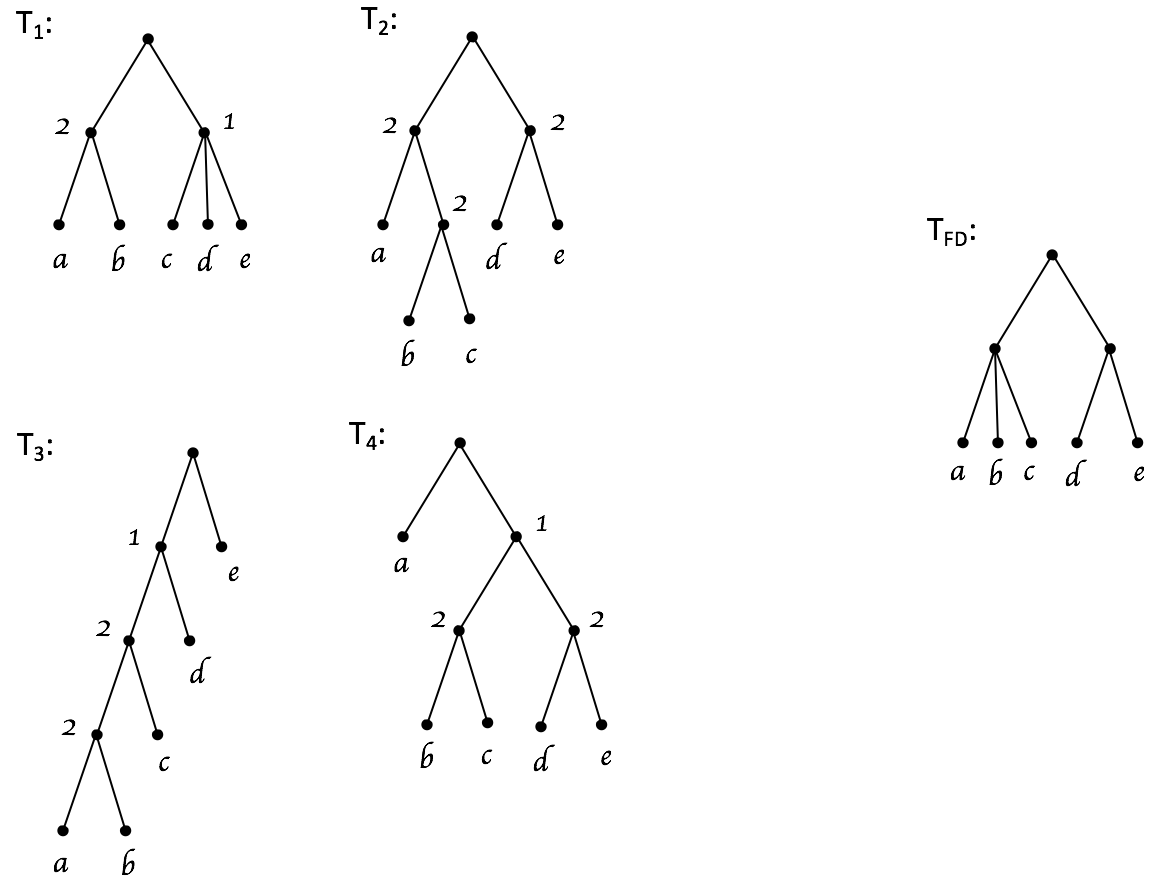
\includegraphics[scale=0.5]{freqdiff}
        \centering
        \caption{Example of a frequency difference consensus tree}
        \label{fig:freqdiff}
    \end{figure}

    Finally, for any tree $T$, define $path^{T}(v, w)$ for any nodes $v, w \in V(T)$ be the set of all nodes that are ancestors of $v$ and proper descendants of $w$. That is, $path^{T}(v, w)$ contains all nodes on the path from $v$ to $w$, excluding $w$. Notice that $path^{T}(v, w) \neq \emptyset$ exactly when $w$ is a proper ancestor of $v$.

    Henceforth, $\mathcal{S}$ is taken to be the input set of trees with identical leaf labels. This set of leaf labels is denoted by $L$. Let $|\mathcal{S}| = k$ and $|L| = n$.

    \subsection{Previous Work}
    Jansson et al. \cite{jansson2018algorithms} gave a deterministic $min\{O(kn^2), O(kn(k + log^2 n))\}$ algorithm for constructing the frequency difference tree. Gawrychowski et al. \cite{gawrychowski2017faster} improved this to a deterministic $O(kn\,log^2n)$ algorithm.

    \subsection{Organisation of the Article and New Results}
    Section~\ref{sec:preliminaries} contains some results from previous works that are utilised later. Section~\ref{sec:freqdiffconstruction} presents a new deterministic algorithm for constructing the frequency difference tree that runs in $O(kn\,log\,n)$ time. Section~\ref{sec:futurework} lays out plans for future work.

    \section{Preliminaries}
    \label{sec:preliminaries}

    \subsection{Centroid Path Decomposition}

    The \textit{centroid path decomposition technique} of \cite{cole2000n} is used to decompose a tree $T$ into a path from root to some leaf and a set of subtrees. A \textit{centroid path} in $T$ is the path formed by starting at the root and at each point following the child with the largest leaf set. The centroid path is denoted by $\pi = \langle p_{\alpha}, p_{\alpha - 1}, ..., p_1 \rangle$, where $p_{\alpha}$ is the root of $T$ and $p_1$ is a leaf. Removing all nodes in $\pi$ along with all associated edges from $T$ results in a set of disjoint subtrees of $T$, where the root of each such subtree is a child of some node in $\pi$. These trees are called the \textit{side trees} of $\pi$, denoted by $\sigma(\pi)$. Also let $\sigma(p_i)$ be the set of side trees whose roots are children of $p_i$, called the side trees \textit{associated} with $p_i$.

    \subsection{The \textit{delete} operation}
    As described in \cite{jansson2018algorithms}, the \textit{delete} operation deletes a cluster from a tree. To do so, we specify some internal node $u$ in a tree $T$, such that we wish $\leafset(T[u])$ to be deleted. Then the \textit{delete} operation makes $parent(u)$ the parent of all nodes in $children(u)$ and removes $u$, along with any associated edges from $T$. This has the effect of removing only $\leafset(T[u])$ from $T$, without affecting any other cluster.

    \subsection{Characterising incompatibility}
    We restate Lemma 6 of \cite{jansson2018algorithms} here since it is crucial in the development of an algorithm discussed below:
    \newline

    \begin{incompatibility}
        \label{lem:incompatibility}

        Given a tree $T$ and a cluster $C \subseteq \leafset(T)$, let $r_C = lca^T(C)$. Then for any $u \in V(T)$, $C \not\compatible \leafset(T[u])$ iff $u$ lies on the path between $r_C$ and some $x \in C$ and $\leafset(T[u]) \not\subseteq C$.
    \end{incompatibility}

    \subsection{\texttt{Frequency\_Difference} algorithm}
    The algorithm \texttt{Frequency\_Difference} is laid out in \cite{jansson2018algorithms}. Before describing this, we first define the weight of a node $u$ to be the number of trees in $\mathcal{S}$ that the cluster associated with $u$ occurs in. Formally, for any tree $T \in \mathcal{S}$ and any node $u \in V(T)$, let $C = \leafset(T[u])$, then $weight(u) = w(u) = |K_C|$ and $w(C) = w(u)$. Further, define a procedure \texttt{Filter\_Clusters} which takes in trees $T_A$ and $T_B$, with $\leafset(T_A) = \leafset(T_B) = L$ and $w(u)$ computed for any $u \in V(T_A) \cup V(T_B)$. It returns a tree $T$ which contains all clusters $C$ in $T_A$ for which $w(C) > $ weight of all clusters in $T_B$ that it is incompatible with. Formally, \texttt{Filter\_Clusters}$(T_A, T_B) = T$ where $\mathcal{C}(T) = \{C : C \in \mathcal{C}(T_A) \text{ and } w(C) > max(\{w(C_1) : C_1 \in \mathcal{C}(T_B) \text{ and } C_1 \not\compatible C\})\}$ and $\leafset(T) = L$.

    Then the algorithm \texttt{Frequency\_Difference} runs in two parts. First, for any tree $T \in \mathcal{S}$ and any node $u \in V(T)$, it computes $w(u)$. We call this the \textit{labelling} step. In the second part, it utilises \texttt{Filter\_Clusters} and \texttt{Merge\_Trees} (from \cite{jansson2016improved}) to compute the frequency difference consensus tree. Theorem 3 of \cite{jansson2018algorithms} gives the following corollary:
    \newline

    \begin{freqdiffruntimecomponents}
        \label{cor:freqdiffruntimecomponents}

        The total runtime of \texttt{Frequency\_Difference} is given by $O(g(n, k) + k \cdot f(n))$ where $g(n, k)$ is the time taken by the labelling step and $f(n)$ is the runtime of \texttt{Filter\_Clusters}.
    \end{freqdiffruntimecomponents}

    Jansson et al. \cite{jansson2018algorithms} gave a $min(\{O(kn^2), O(k^2n)\})$ solution to the labelling step and an $O(n\,log^2n)$ solution to \texttt{Filter\_Clusters}, giving an overall runtime of $min(\{O(kn^2), O(kn(k + log^2n))\})$. Gawrychowski et al. \cite{gawrychowski2017faster} improved the runtime of the labelling step to $O(kn\,log^2n)$, thus reducing the overall runtime to $O(kn\,log^2n)$.

    \section{RMQ (range minimum/maximum query) structure on trees}
    \label{sec:rmqstructure}

    This section presents a way to build an RMQ structure on a tree $T$. We assume that for every node $u \in V(T)$, some property $weight(u)$ is defined. Then we build a structure capable of answering the query, for any $v, w \in V(T)$, $max_{u \in path^{T}(v, w)}(weight(u))$ in constant time. Recall that $path^{T}(v, w)$ is the set of nodes on the path from $v$ to $w$, excluding $w$.

    Lemma 8 of \cite{jansson2018algorithms} presents a way to build this RMQ structure where queries include the node $w$. These queries are represented by $rmq(v, w)$. We first elaborate on their solution to show how to implement a key step in their procedure. Then we give a way to find the child of $w$ which is also an ancestor of $v$, refererred to as $childForDescendant(w, v)$ in constant time. Then $max_{u \in path^{T}(v, w)}(weight(u)) = rmq(v, childForDescendant(w, v))$.

    \subsection{Answering $rmq(v, w)$}
    \label{subsec:answeringrmq}

    Lemma 8 of \cite{jansson2018algorithms} first decomposes $T$ into a centroid path and a set of side trees, each of which is recursively partitioned, giving a set of centroid paths. Let this set be $P$. The linear RMQ structure of \cite{bender2000lca} is used to store each of these. Then for each $x \in \leafset(T)$, they denote the centroid \textit{subpaths} on the path from $x$ to the root of $T$ by $Q_1, Q_2, ..., Q_f$ and build the array $W_x[1 ... f]$ where $W_x[i] = max_{u \in Q_i}(weight(u))$. Each $W_x$ is stored in a linear RMQ structure.

    Now to find $rmq(v, w)$, consider the path from $v$ to $w$. This can again be seen as a concatenation of subpaths of centroid paths, say $Q_1, Q_2, ..., Q_g$. Let $x \in \leafset(v)$. Then $Q_2, ..., Q_{g - 1}$ are contained fully on the path from $x$ to $root(T)$. $Q_1$ must be a subpath that starts at some node ($v$) in a centroid path $\in P$ and ends at the root of that centroid path. $Q_g$ is a subpath that starts at some node in some centroid path $\in P$ and ends at another node within the same path ($w$). We address each of these three divisions separately.

    To find the maximum weight within $Q_1$, we augment each node with its depth within its centroid path. This is easy to do during the decomposition. Then we can retreive the maximum weight by querying the linear RMQ structure for this centroid path, from the root to $v$.

    To find the maximum weight for the subpaths $Q_2, ..., Q_{g - 1}$, we augment each centroid path with its ``depth''. This is defined as the number of roots of centroid paths that are above the root of the given centroid path in the tree. Intuitively, if we build a tree from only the roots of the centroid paths while maintaining the same relative structure, then the depth of a centroid path would simply be the depth of its root in this new tree. Again, these depths are easy to obtain during the decomposition. Then the indices of $Q_2$ and $Q_{g-1}$ in $W_x$ can be found using the depths of $Q_1$ and $Q_{g - 1}$ respectively.

    Finally, we need to find the maximum weight within $Q_g$. Observe that the key here is finding which node is at the end of $Q_g$. This is equivalent to finding which node in the centroid path of which $Q_g$ is a subpath has $x$ in one of its side trees. We first number the leaves of $T$ such that for any $P_i \in P$, for any nodes $r, s \in P_i$ where $depth(r) < depth(s)$, all leaves in the side trees associated with $r$ have a higher index than any leaf in the side trees associated with $s$. This can be done by traversing centroid paths from bottom to top, recursively indexing the side trees, and then starting the indexing for the next set of side trees where the previous set left off. Now for each $P_i \in P$, we do the following. For each node in $P_i$, we find the minimum index of all the leaves in its side trees and store these in the succinct data structure of \cite{jacobson1988succinct}. This data structure supports rank queries in constant time. Thus, we can find the desired ending node of $Q_g$ in constant time, by querying for the rank of $x$ in the succinct data structure for the centroid path containing $Q_g$. The linear RMQ structure for this centroid path can then give us the maximum weight within $Q_g$.

    A succinct data structure takes $O(n)$ preprocessing time, where $n$ is the range of the numbers being stored in the structure. Thus, for a centroid path rooted at $p_{\alpha}$, the amount of time taken to construct the succinct structure is proportional to $|\leafset(p_{\alpha})|$ since leaves in the side trees are consecutively numbered. By the standard argument of heavy-path decomposition, each leaf belongs to $O(log\,n)$ centroid paths and so total time to construct all the succinct structures is $O(n\,log\,n)$. Further, the other operations outlined above also take $O(n\,log\,n)$ preprocessing time (including the work done in Lemma 8 of \cite{jansson2018algorithms}), and together allow answering $rmq(v, w)$ in constant time.

    \subsection{Answering $childForDescendant(v, w)$}
    \label{subsec:answeringcfd}

    As in Subsection~\ref{subsec:answeringrmq}, we decompose $T$ into a set of centroid paths. A $childForDescendant(v, w)$ can now be divided into first checking if the heavist child of $w$ is an ancestor of $v$, and if not, then finding out which of the other children of $w$ is an ancestor of $v$.

    To solve the first problem, we assign each leaf an index in left to right order and augment each node with the index of its leftmost and rightmost leaves. Then to check if a node $r$ is an ancestor of a node $s$, we simply need to verify that the leftmost leaf of $s$ is not to the left of the leftmost leaf of $r$, and similarly with their rightmost leaves. This takes constant time.

    To solve the second problem, we index the leaves as in Subsection~\ref{subsec:answeringrmq}. Now for each node we create a succinct data structure storing the smallest leaf index for each of its children (excluding the heavist child). Then finding out which of the children is an ancestor of $v$ can be done by querying for the rank of any leaf $x \in \leafset(T[v])$ in the succint structure of $w$ (in constant time). Again, by a heavy-path decomposition argument, it can be seen that any leaf contributes to $O(log\,n)$ succint structures, and so total time to construct these is $O(n\,log\,n)$.
    \newline

    \begin{rmqstructure}
        \label{theorem:rmqstructure}
        A query of the form $max_{u \in path^{T}(v, w)}(weight(u))$ can be answered in $O(1)$ time with $O(n\,log\,n)$ preprocessing time.

        \begin{proof}
            Follows from the arguments above.
        \end{proof}
    \end{rmqstructure}

    \section{Constructing the Frequency Difference Consensus Tree}
    \label{sec:freqdiffconstruction}

    We present an $O(kn\,log\,n)$ solution for the labelling step in section 3.1 and an $O(n\,log\,n)$ solution for \texttt{Filter\_Clusters} in section 3.2. Taken together with Corollary 2, this allows us to solve \texttt{Frequency\_Difference} in $O(kn\,log\,n)$ time.

    \subsection{Labelling}
    As in \cite{gawrychowski2017faster}, we divide the labelling step into two parts. First, we give a label to every node $u$, where $u \in V(T)$ for some $T \in \mathcal{S}$, denoted by $id(u)$. The labels obey the restrictions that $id(u) \in [1, 2kn]$ and for some $u' \in T'$, $T' \in \mathcal{S}$, $id(u) = id(u')$ iff $\leafset(T[u]) = \leafset(T'[u'])$. That is, two nodes will have the same label iff they are associated with the same cluster. Second, we counting sort these labels, allowing us to count how many nodes exist with a certain label, giving us the frequency of those nodes in $\mathcal{S}$.

    First, for some tree $T$ and some cluster $C \subseteq \leafset(T)$ define $T|C$, read as ``$T$ restricted to $C$'', as the tree $T'$ with $V(T') = \{lca^T(u, v) : u, v \in C\}$ which obeys $lca^T(C') = lca^{T'}(C')$ for all nonempty $C' \subseteq C$. Intuitively, $T'$ has the leaf set $C$ and consists of all nodes in $T$ that are $lca$'s of the leafs in $C$, with these nodes connected such that they have the same ancestor/descendant relationships as they had in $T$. Further, for any node $u$ in $T$, define the node that $u$ is associated with when $T$ is restricted to $C$ to be the descendant of $u$ with least depth that is in $T|C$, denoted as $assoc^{C}(u)$. If no such node exists, then define for convenience a node with an empty leaf set and id $0$.

    The algorithm \texttt{Label\_Clusters} is laid out below.

    \begin{algorithm}
        \caption{Label\_Clusters}
        \label{alg:labelclusters}

        \begin{algorithmic}[1]
            \Input A set $\mathcal{S}$ of trees $\{T_1, T_2, ..., T_k\}$ where $\leafset(T_1) = \leafset(T_2) = ... = \leafset(T_k) = L$

            \Output Every node in the trees in $\mathcal{S}$ is labelled such that nodes associated with the same cluster have the same labels and for any node $u$, $id(u) \in [1, 2k |L|]$

            \State Partition $L$ into $L'$ and $L''$ such that $|L'| = |L''|$.

            \State For all $i \in [1,k]$, let $T'_i = T_i|L'$ and $T''_i = T_i|L''$.

            \State \texttt{Label\_Clusters}$(T'_1, T'_2, ..., T'_k)$.

            \State \texttt{Label\_Clusters}$(T''_1, T''_2, ..., T''_k)$.

            \State For every tree $T \in \mathcal{S}$, for every node $u \in T$, represent $u$ by the pair $(id(assoc^{L'}(u)), id(assoc^{L''}(u)))$.

            \State Radix sort all pairs obtained. Assign each set of duplicates found thus a rank.

            \State For every tree $T \in \mathcal{S}$, for every node $u \in T$, set $id(u) = $ rank of the pair $(id(assoc^{L'}(u)), id(assoc^{L''}(u)))$.
        \end{algorithmic}
    \end{algorithm}

    One iteration of this process is illustrated in Figure~\ref{fig:labelclusters}. Here $L' = \{a, b, c, d\}$ and $L'' = \{e, f, g, h\}$. It is assumed that the algorithm has correctly labelled the clusters for each of the restricted trees, and these labels are assigned as shown. $T_1$ and $T_2$ then show the pair associated with each internal node. For example, the cluster $\{a, b, e\}$ in $T_1$ is labelled by $5$ from $\{a, b\}$ in $T_1|L'$ and $1$ from $\{e\}$ in $T_1|L''$.

    \begin{figure}[h]
        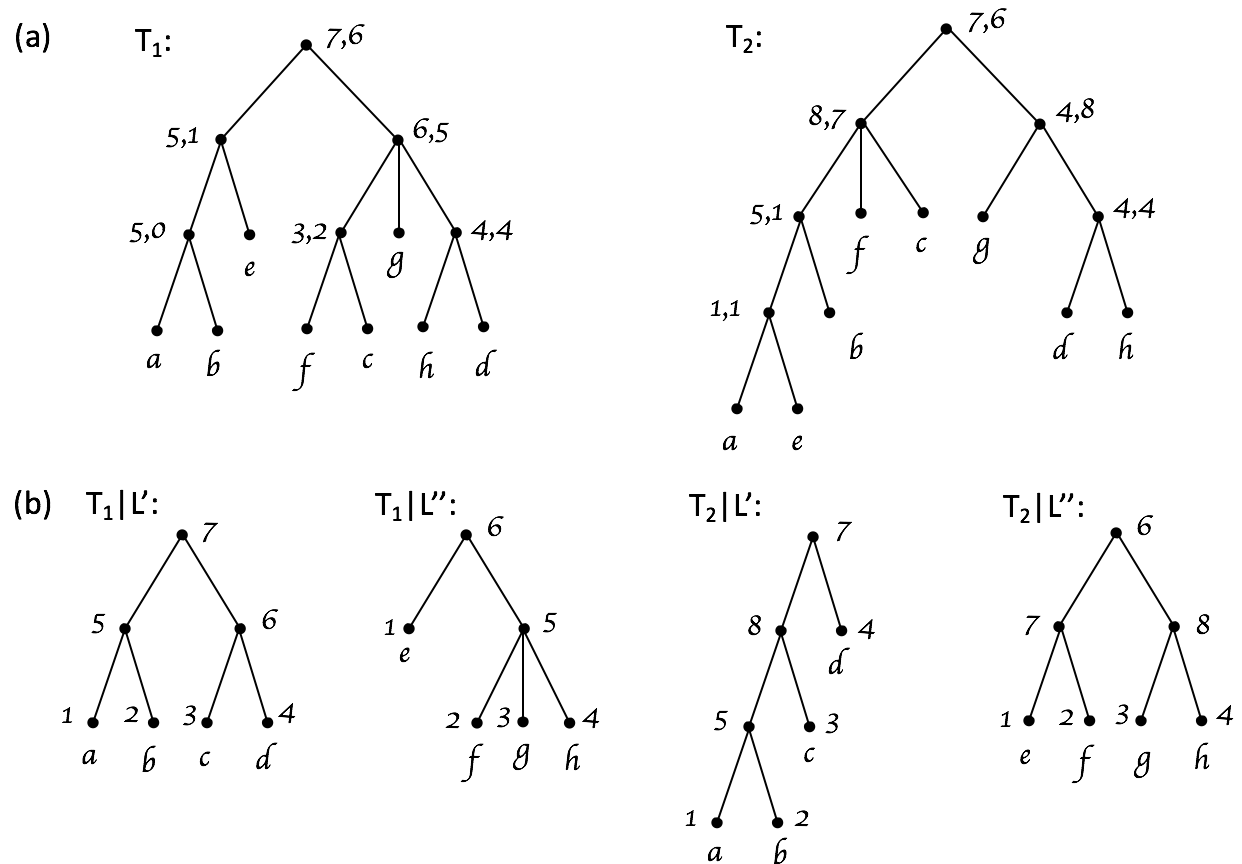
\includegraphics[scale=0.5]{labelclusters}
        \centering
        \caption{Demonstration of \texttt{Label\_Clusters}}
        \label{fig:labelclusters}
    \end{figure}

    \bigskip
    \begin{assocnode}
        \label{lem:assocnode}

        For any tree $T$, for any node $u \in V(T)$ and any cluster $C \subseteq \leafset(T)$, $\leafset(T|C[assoc^C(u)]) = \leafset(T[u])\, \cap\, C$.

        \begin{proof}
            First note that for any node $v \in V(T|C)$, $\leafset(T|C[v]) = \leafset(T[v])\, \cap\, C$ due to the way $T|C$ is constructed. Also, $\leafset(T[assoc^C(u)]) \subseteq \leafset(T[u])$ since $assoc^C(u)$ is a descendant of $u$. Thus $\leafset(T[assoc^C(u)])\, \cap\, C \subseteq \leafset(T[u])\, \cap\, C$ and so $\leafset(T|C[assoc^C(u)]) \subseteq \leafset(T[u])\, \cap\, C$.

            This implies that if $\leafset(T|C[assoc^C(u)]) \neq \leafset(T[u])\, \cap\, C$ then there is some leaf $x$ such that $x \in \leafset(T[u])\, \cap\, C$ and $x \not\in \leafset(T|C[assoc^C(u)])$. Then let $v = lca^T(C \cup x)$. Observe that $v$ is proper ancestor of $u$, since $\leafset(T[u]) = C \subseteq C \cup x = \leafset(T[v])$ and $\leafset(T[u]) \neq \leafset(T[v])$. Also, since $v = lca^T(C \cup x)$ and $C \cup x \subseteq \leafset(T[u])$, $v$ is a descendant of $u$. Finally, $v \in V(T|C)$. But then an ancestor of $v$ would be $assoc^C(u)$, and not the node that was initially obtained.
        \end{proof}
    \end{assocnode}

    \medskip
    \begin{labelclusterscorrectness}
        \label{lem:labelclusterscorrectness}

        After running \texttt{Label\_Clusters}$(\mathcal{S})$, for any trees $T_i, T_j \in \mathcal{S}$, for any nodes $u \in V(T_i), v \in V(T_j)$, $id(u) = id(v)$ iff $\leafset(T_i[u]) = \leafset(T_j[v])$.

        \begin{proof}
            $id(u) = id(v)$ iff $id(assoc^{L'}(u)) = id(assoc^{L'}(v))$ and $id(assoc^{L''}(u)) = id(assoc^{L''}(v))$. Inductively, the first part is true iff $\leafset(T_i|L'[assoc^{L'}(u)]) = \leafset(T_j|L'[assoc^{L'}(v)])$. By Lemma~\ref{lem:assocnode}, $\leafset(T_i[u])\, \cap\, L' = \leafset(T_j[v])\, \cap\, L'$. Symmetrically, the second part is true iff $\leafset(T_i[u])\, \cap\, L'' = \leafset(T_j[v])\, \cap\, L''$. Since $L'$ and $L''$ partition $L$, both parts are true iff $\leafset(T_i[u]) = \leafset(T_j[v])$.
        \end{proof}
    \end{labelclusterscorrectness}

    \medskip
    \begin{labelclustersidbounds}
        \label{lem:labelclustersidbounds}

        After running \texttt{Label\_Clusters}$(\mathcal{S})$, for any tree $T \in \mathcal{S}$, for any node $u \in V(T)$, $id(u) \in [1, 2k |L|]$.

        \begin{proof}
            $|V(T)| < 2|L|$. Thus the total number of pairs is less than $2k|L|$. This also places an upper bound on the number of ids. Notice that $u$ cannot be labelled with $0$ since that is reserved for the special node.
        \end{proof}
    \end{labelclustersidbounds}

    \medskip
    \begin{labelclustersruntime}
        \label{lem:labelclustersruntime}

        The algorithm \texttt{Label\_Clusters}$(\mathcal{S})$ runs in $O(kn\,log\,n)$ time.

        \begin{proof}
            Let $T(m)$ be the runtime of \texttt{Label\_Clusters}$(\mathcal{T})$, where $m =$ size of leaf set of each tree in $\mathcal{T}$. By Lemma 5.2 of \cite{farach1995fast}, construction of $T'_i$ and $T''_i$ takes $O(m)$ time for each $T_i \in \mathcal{T}$, taking total $O(km)$ time over all the trees. For each $T_i \in \mathcal{T}$, $|V(T_i)| < O(m)$. Computing $assoc^{L'}(u)$ and $assoc^{L''}(u)$ for each node $u$ in some tree $T_i \in \mathcal{T}$ can be done by a bottom up traversal of $T_i$ along with $T'_i$ and $T''_i$, taking $O(km)$ time total. Also observe that the number of pairs obtained is $O(km)$. Further, each of the values in the pair are in the range [0, km]. Thus radix sorting these pairs and assigning labels back to the nodes takes $O(km)$ time. So $T(m) = 2T(m/2) + O(km)$, giving $T(n) = kn\,log\,n$.
        \end{proof}
    \end{labelclustersruntime}

    \subsection{\texttt{Filter\_Clusters}}

    Recall that \texttt{Filter\_Clusters}$(T_A, T_B) = T$ where $\mathcal{C}(T) = \{C : C \in \mathcal{C}(T_A) \text{ and } w(C) > max(\{w(C_1) : C_1 \in \mathcal{C}(T_B) \text{ and } C_1 \not\compatible C\})\}$ and $\leafset(T) = L$. Thus, for any node $u \in V(T_A)$, we would like to find the set of nodes in $T_B$ that are incompatible with $u$, so that we can find the maximum weight of these.

    Before describing how this is done, we prove some important lemmas.
    \newline

    \begin{filterclusterssubsetcompatible}
        \label{lem:filterclusterssubsetcompatible}

        Let nodes $u \in V(T_A)$, $v \in V(T_B)$ such that $\leafset(T_B[v]) \subseteq \leafset(T_A[u])$. Then for any $u' \in V(T_A) - V(T_A[u])$, and any $v' \in V(T_B[v])$, $\leafset(T_A[u']) \compatible \leafset(T_B[v'])$.

        \begin{proof}
            Note that $\leafset(T_B[v']) \subseteq \leafset(T_B[v])$ since $v'$ is in the subtree rooted at $v$. There are two cases for $u'$. \textit{Case 1}: $u'$ is an ancestor of $u$. Then $\leafset(T_A[u]) \subseteq \leafset(T_A[u'])$. Thus $\leafset(T_B[v']) \subseteq \leafset(T_A[u'])$, and so $\leafset(T_B[v']) \compatible \leafset(T_A[u'])$. \textit{Case 2}: $u'$ is not an ancestor of $u$. Since $u'$ is also not a descendant of $u$, $\leafset(T_A[u']) \cap \leafset(T_A[u]) = \emptyset$. Thus $\leafset(T_A[u']) \cap \leafset(T_B[v']) = \emptyset$ and so $\leafset(T_B[v']) \compatible \leafset(T_A[u'])$.
        \end{proof}
    \end{filterclusterssubsetcompatible}

    This lemma says that if the cluster associated with some node $v \in V(T_B)$ is a subset of the cluster associated with some node $u \in V(T_A)$, then $v$ is the root of a subtree of $T_B$ that is compatible with every node in $V(T_A) - V(T_A[u])$. The upshot of this is that if once we process $u$ we are known to have also processed the entirety of $T_A[u]$, then for the remaining nodes, no node in $V(T_B[v])$ needs to be considered for incompatibility again.

    For any cluster $C \subseteq L$, define any node $r \in V(T_B)$ to be the root of a \textit{maximal subtree compatible with $C$} if it satisfies the following property: $\leafset(T_B[r]) \subseteq C$ and there is no proper ancestor $r'$ of $r$ such that $\leafset(T_B[r']) \subseteq C$. The set $rootsOfSubtrees(C)$ is composed of all nodes $r \in V(T_B)$ that are roots of maximal subtrees compatible with $C$.

    We now prove a stronger version of Lemma~\ref{lem:incompatibility} that takes $rootsOfSubtrees$ into account to compute the set $incompatible(u) = \{v : v \in V(T_B) \text{ and } \leafset(T_B[v]) \not\compatible \leafset(T_A[u])\}$ for any $u \in V(T_A)$.
    \newline

    \begin{incompatibilityrootsofsubtrees}
        \label{lem:incompatibilityrootsofsubtrees}

        Let $path(v, w)$ for any nodes $v, w \in T_B$ be a set containing all nodes that are ancestors of $v$ and proper descendants of $w$. For any node $u \in V(T_A)$, define $l_u = lca^{T_B}(\leafset(T_A[u]))$. Then for any $u \in V(T_A)$, $v \in incompatible(u)$ iff $v$ is a proper descendant of $l_u$ and for some $r \in rootsOfSubtrees(u)$, $v$ is a proper ancestor of $r$. i.e. $incompatible(u) = \bigcup_{r \in rootsOfSubtrees(u)} path(parent^{T_B}(r), l_u)$.

        \begin{proof}
            \textit{Forward direction}: Given some $v \in V(T_B)$ such that $\leafset(T_B[v]) \not\compatible \leafset(T_A[u])$, $v$ must be a proper descendant of $l_u$ by Lemma~\ref{lem:incompatibility}. Further, for some $x \in \leafset(T_A[u])$, $v$ is a proper ancestor of $x$ by Lemma~\ref{lem:incompatibility}. Then there must be $r \in rootsOfSubtrees(u)$, $r$ is an ancestor of $x$. $v \not\in V(T_B[r])$, otherwise $\leafset(T_B[v]) \subseteq \leafset(T_A[u])$. Thus $v$ is a proper ancestor of $r$.

            \textit{Backward direction}: Given some $v \in V(T_B)$ such that $v$ is a proper descendant of $l_u$ and for some $r \in rootsOfSubtrees(u)$, $v$ is a proper ancestor of $r$. Since $v$ is a proper descendant of $l_u$, $\leafset(T_A[u]) \not\subseteq \leafset(T_B[v])$. Since $v$ is a proper ancestor of $r$, $\leafset(T_B[r]) \subset \leafset(T_B[v])$, so $\leafset(T_B[v]) \cap \leafset(T_A[u]) \neq \emptyset$. Finally, $\leafset(T_B[v]) \not\subseteq \leafset(T_A[u])$, otherwise $r \not\in rootsOfSubtrees(u)$.
        \end{proof}
    \end{incompatibilityrootsofsubtrees}

    This is illustrated in Figure~\ref{fig:rootsofsubtrees}. Here, any node in $rootsOfSubtrees(\{a, b, c, f, g, h\})$ is circled and any node that is incompatible with this cluster has a rectangle around it.

    \begin{figure}[h]
        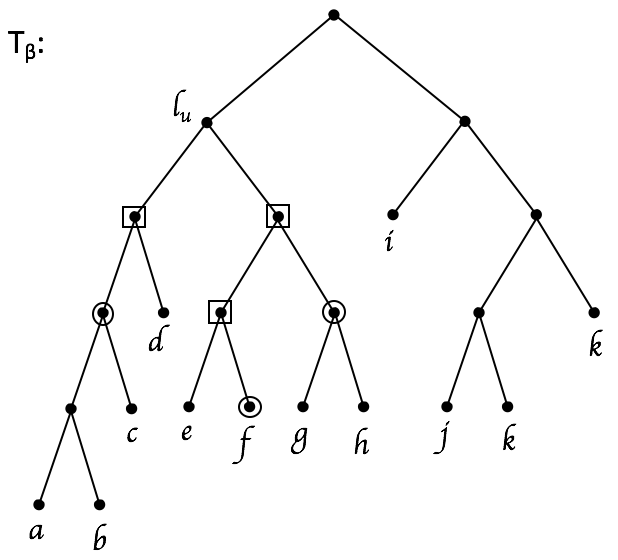
\includegraphics[scale=0.5]{rootsofsubtrees}
        \centering
        \caption{Illustration of Lemma~\ref{lem:incompatibilityrootsofsubtrees}}
        \label{fig:rootsofsubtrees}
    \end{figure}

    We now build a recursive definition of $incompatible(u)$, for any internal node $u \in V(T_A)$. To do so, we use $incompatible(c_1)$, for some $c_1 \in children(u)$.
    \newline

    \begin{incompatibilityrecursive}
        \label{lem:incompatibilityrecursive}

        Given any internal node $u \in V(T_A)$ and $c_1 \in children(u)$, define
        \begin{align*}
            newRootsOfSubtrees(u, c_1) &= rootsOfSubtrees(\leafset(T_A[u])) - rootsOfSubtrees(\leafset(T_A[c_1]))\\[0.5em]
            removedRootsOfSubtrees(u, c_1) &= rootsOfSubtrees(\leafset(T_A[c_1])) - rootsOfSubtrees(\leafset(T_A[u]))\\[0.5em]
            oldRootsOfSubtrees(u, c_1) &= rootsOfSubtrees(\leafset(T_A[u])) \cap rootsOfSubtrees(\leafset(T_A[c_1]))
        \end{align*}
        Then for any $r_1 \in oldRootsOfSubtrees(u, c_1)$ (if this does not exist then the relevant term below is empty),
        \begin{align*}
            incompatible(u) = &\left(incompatible(c_1)\ -\ \bigcup_{r \in removedRootsOfSubtrees(u, c_1)} path(parent^{T_B}(r), l_{c_1})\right)\\
            &\cup\ \bigcup_{r \in newRootsOfSubtrees(u, c_1)} path(parent^{T_B}(r), l_u)\\
            &\cup\ path(parent^{T_B}(r_1), l_u)
        \end{align*}

        \begin{proof}
            The intuition behind this is to see that nodes that are proper ancestors of any $r \in removedRootsOfSubtrees(u, c_1)$ and descendants of any $r' \in newRootsOfSubtrees(u, c_1)$ need to be removed from $incompatible(c_1)$ since they are compatible with $u$. This accounts for the first two lines in the statement. The last line is to ensure that nodes between $l_{c_1}$ and $l_u$ are added to the set of incompatible nodes if necessary.

            First, it must be true that for any $r \in removedRootsOfSubtrees(u, c_1)$, there is some $r' \in newRootsOfSubtrees(u, c_1)$ such that $r'$ is a proper ancestor of $r$. If not, then we note that $\leafset(T_B[r]) \subseteq \leafset(T_A[c_1]) \subseteq \leafset(T_A[u])$ and there is no ancestor $r''$ of $r$ such that $\leafset(T_B[r'']) \subseteq \leafset(T_A[u])$, thus $r \in rootsOfSubtrees(\leafset(T_A[u]))$. But then $r \not\in removedRootsOfSubtrees(u, c_1)$.

            \textit{Forward direction.} Let $v \in incompatible(u)$. Then by Lemma~\ref{lem:incompatibilityrootsofsubtrees}, $v$ is a proper descendant of $l_u$. If there is some $r \in newRootsOfSubtrees(u, c_1)$ such that $v$ is a proper ancestor of $r$ then $v \in path(parent^{T_B}(r), l_u)$. Otherwise, by Lemma~\ref{lem:incompatibilityrootsofsubtrees}, there must be some $r \in oldRootsOfSubtrees(u, c_1)$ such that $v$ is a proper ancestor of $r$. Then for all $r' \in removedRootsOfSubtrees(u, c_1)$, it cannot be that $v$ is a proper ancestor of $r'$. To see why, assume this is not true, i.e. there is some $r' \in removedRootsOfSubtrees(u, c_1)$ such that $v$ is a proper ancestor of $r'$. Then there is some $r'' \in newRootsOfSubtrees(u, c_1)$ such that $r''$ is a proper ancestor of $r'$. If $v$ is a descendant of $r''$, then $\leafset(T_B[v]) \subseteq \leafset(T_B[r'']) \subseteq \leafset(T_A[u])$. But then $v \not\in incompatible(u)$. Otherwise, if $v$ is a proper ancestor of $r''$, then there is some $r'' \in newRootsOfSubtrees(u, c_1)$ such that $v$ is a proper ancestor of $r''$, which contradicts our earlier assumption. Thus is $v$ is a proper descendant of $l_{c_1}$, then $v \in incompatible(c_1)\ -\ \bigcup_{r \in removedRootsOfSubtrees(u, c_1)} path(parent^{T_B}(r), l_{c_1}$. Otherwise, $v \in path(parent^{T_B}(r_1), l_u)$ since $path(l_{c_1}, l_u) \subseteq path(parent^{T_B}(r_1), l_u)$.

            \textit{Backward direction.} Let $v \in RHS$ of equation above.

            \textit{Case 1.} $v \in \bigcup_{r \in newRootsOfSubtrees(u, c_1)} path(parent^{T_B}(r), l_u)$. Then by Lemma~\ref{lem:incompatibilityrootsofsubtrees}, $v \in incompatible(u)$.

            \textit{Case 2.} $v \in path(parent^{T_B}(r_1), l_u)$. Since $r_1 \in rootsOfSubtrees(\leafset(T_A[u]))$, by Lemma~\ref{lem:incompatibilityrootsofsubtrees}, $v \in incompatible(u)$.

            \textit{Case 3.} $v \in incompatible(c_1)\ -\ \bigcup_{r \in removedRootsOfSubtrees(u, c_1)} path(parent^{T_B}(r), l_{c_1})$ and $v \not\in \bigcup_{r \in newRootsOfSubtrees(u, c_1)} path(parent^{T_B}(r), l_u)$. Since $v \in incompatible(c_1)$, it is easy to see that $\leafset(T_B[v]) \cap \leafset(T_A[u]) \neq \emptyset$ and $\leafset(T_A[u]) \not\subseteq \leafset(T_B[v])$. Also, there is some leaf $x \in \leafset(T_B[v])$ such that $x \not\in \leafset(T_A[c_1])$. If $x \in \leafset(T_A[u])$, then there is some $r \in rootsOfSubtrees(\leafset(T_A[u]))$ such that $r$ is an ancestor of $x$. Then $r \in newRootsOfSubtrees(u, c_1)$ since $x \in \leafset(T_B[r])$ and $x \not\in \leafset(T_A[c_1])$. We also note that $v$ is an ancestor of $x$. If $v$ is a proper ancestor of $r$, then $v \in path(parent^{T_B}(r), l_u)$, which contradicts the definition of $v$. Thus $v$ is a descendant of $r$. Since $v \in incompatible(c_1)$, there is some $r' \in rootsOfSubtrees(\leafset(T_A[c_1]))$ such that $v$ is a proper ancestor of $r'$. But then $r$ is a proper ancestor of $r'$, so $r' \not\in rootsOfSubtrees(\leafset(T_A[u]))$. Thus $r \in removedRootsOfSubtrees(u, c_1)$. But then $v \in \bigcup_{r \in removedRootsOfSubtrees(u, c_1)} path(parent^{T_B}(r), l_{c_1})$. Thus $x \not\in \leafset(T_A[u])$ and so $v \in incompatible(u)$.
        \end{proof}
    \end{incompatibilityrecursive}

    Figure~\ref{fig:incompatibilityrecursive} illustrates the above result. Here $rootsOfSubtrees(c_1) = \{r_1, r_2\}$ and $rootsOfSubtrees(u) = \{r_1, r_3, r_4, r_5\}$. The triangles under each of these nodes represent the subtrees rooted at them. The nodes on the dotted line between $r_1$ and $l_{c_1}$ are in $incompatible(c_1)$ and remain in $incompatible(u)$. The nodes on the dashed line between $r_2$ and $r_4$ are now known to be compatible with $u$, so they will be removed from $incompatible(c_1)$. The nodes on the bold lines from $r_3$, $r_4$ and $r_5$ are added to $incompatible(c_1)$ to get $incompatible(u)$. Notice that the nodes between $l_{c_1}$ and $l_u$ are added due to $r_3$ and $r_4$, but even if no root of a maximal subtree compatible with $\leafset(T_A[u])$ is in $V(T_B[l_{c_1}])$, these nodes would have been added due to $r_1$, which belongs to $oldRootsOfSubtrees(u, c_1)$.

    \begin{figure}[h]
        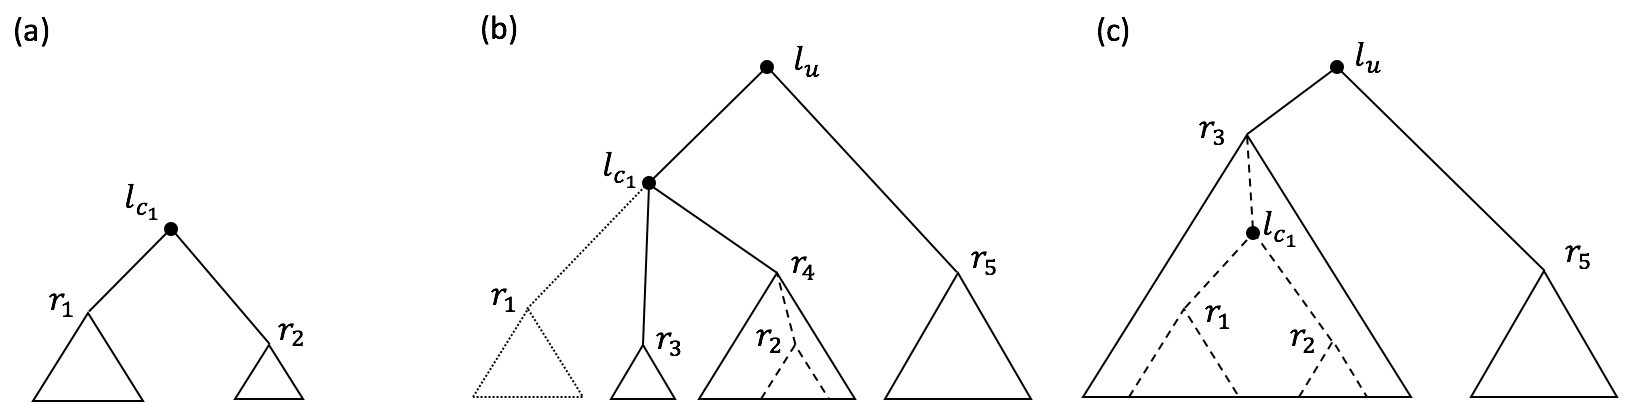
\includegraphics[scale=0.5]{incompatibilityrecursive}
        \centering
        \caption{Illustration of Lemma~\ref{lem:incompatibilityrecursive}}
        \label{fig:incompatibilityrecursive}
    \end{figure}

    We also define a property $counter(v)$ for any $v \in T_B$ (as in \cite{jansson2018algorithms}). $T_B$ satisfies the parent counter invariant for some cluster $C \subseteq L$, denoted as $pci(C)$, iff for all nodes $v \in \bigcup_{r \in rootsOfSubtrees(C)} parent^{T_B}(r)$, $counter(v) = |children(v) \cap rootsOfSubtrees(C)|$.

    We thus present Algorithm~\ref{alg:computerootsofsubtrees}, which, for some internal node $u \in V(T_A)$ and $c_1 \in children(u)$, takes in $rootsOfSubtrees(c_1)$, $lowerBoundary(u, c_1) = \bigcup_{c \in children(u) - \{c_1\}} rootsOfSubtrees(\leafset(T_A[c]))$ and $T_B$ where $pci(\leafset(T_A[c_1]))$ holds and returns $newRootsOfSubtrees(u, c_1)$, $removedRootsOfSubtrees(u, c_1)$ and $oldRootsOfSubtrees(u, c_1)$. In addition $T_B$ is updated so that $pci^{T_B}(\leafset(T_A[u]))$.

    The algorithm iterates upwards from each node in $lowerBoundary$, updating $counter$ values, and in doing so discovering which nodes are compatible with $\leafset(T_A[u])$. We prove the correctness of this algorithm below.

    \begin{algorithm}
        \caption{Compute\_Roots\_Of\_Subtrees}
        \label{alg:computerootsofsubtrees}

        \begin{algorithmic}[1]
            \Input For some internal node $u \in V(T_A)$ and $c_1 \in children(u)$, $rootsOfSubtrees(c_1)$, $lowerBoundary(u, c_1)$ and $T_B$ where $pci(\leafset(T_A[c_1]))$ holds with $\leafset(T_A) = \leafset(T_B) = L$.

            \Output $newRootsOfSubtrees(u, c_1)$, $removedRootsOfSubtrees(u, c_1)$ and $oldRootsOfSubtrees(u, c_1)$.

            \SideEffect $pci(\leafset(T_A[u]))$ holds.

            \State $new, removed := \{\}$

            \ForAll{$v \in lowerBoundary(u, c_1)$}
                \State $counter(parent^{T_B}(v)) := counter(parent^{T_B}(v)) + 1$

                \State $v := parent^{T_B}(v)$

                \While{$counter(v) = |children(v)|$}
                    \State $counter(parent^{T_B}(v)) := counter(parent^{T_B}(v)) + 1$

                    \State $new := (new \cup \{v\}) - children(v)$

                    \State $removed := removed \cup (children(v) \cap rootsOfSubtrees(c_1))$

                    \State $v := parent^{T_B}(v)$
                \EndWhile
            \EndFor

            \State $newRoots := new$

            \State $removedRoots := removed$

            \State $oldRoots := rootsOfSubtrees(c_1) - removed$

            \State \Return $newRoots$, $removedRoots$, $oldRoots$
        \end{algorithmic}
    \end{algorithm}

    \bigskip
    \begin{computerootsofsubtreescorrectness}
        \label{lem:computerootsofsubtreescorrectness}

        For any internal node $u \in V(T_A)$ and $c_1 \in children(u)$, the algorithm \texttt{Compute\_Roots\_Of\_Subtrees}$(rootsOfSubtrees(c_1), lowerBoundary(u, c_1), T_B)$ outputs $newRootsOfSubtrees(u, c_1)$, $removedRootsOfSubtrees(u, c_1)$ and $oldRootsOfSubtrees(u, c_1)$.

        \begin{proof}
            We prove a loop invariant. Let the nodes in $lowerBoundary$ be numbered $1$ to $\beta = |lowerBoundary|$ in the order that they will be iterated over, i.e. $lowerBoundary = \{r_1, r_2, ..., r_{\beta}\}$. We define $D_0 = \leafset(T_A[c_1])$ for convenience. For any $i$, $1 \leq i \leq \beta$, let $D_i = D_0 \cup \bigcup_{j = 1}^{i} \leafset(T_B[r_j])$. Define $new_i = rootsOfSubtrees(D_i) - rootsOfSubtrees(D_0)$ and $removed_i = rootsOfSubtrees(D_0) - rootsOfSubtrees(D_i)$. Then we claim that after the loop in \texttt{Compute\_Roots\_Of\_Subtrees} is finished processing $r_i \in lowerBoundary$, the sets $new = new_i$ and $removed = removed_i$. Additionally, $pci(D_i)$ holds. Notice that the base case holds trivially.

            We consider the loop for $r_i \in lowerBoundary$. First, observe the following properties of $new_i$ and $removed_i$.

            \textit{$new_i - new_{i-1}$.} Take any $r \in new_i - new_{i-1}$. Then $r \in rootsOfSubtrees(D_i) - rootsOfSubtrees(D_{i-1}) - rootsOfSubtrees(D_0)$. Since $r \in rootsOfSubtrees(D_i) - rootsOfSubtrees(D_{i-1})$, $\leafset(T_B[r]) \subseteq D_i$ and $\leafset(T_B[r]) \not\subseteq D_{i-1}$. Thus there is some $x \in \leafset(T_B[r])$ such that $x \in D_i - D_{i-1}$. Note that $r$ is an ancestor of $x$. $r_i$ is also an ancestor of $x$ since $x \in D_i - D_{i-1} = \leafset(T_B[r_i])$. But $\leafset(T_B[r_i]) \subseteq D_i$. Then $r$ must be an ancestor of $r_i$ since $r \in rootsOfSubtrees(D_i)$. Moreover, there can only be one such $r$, otherwise the definition of $rootsOfSubtrees(D_i)$ would be violated. As $D_i \neq D_{i-1}$, clearly $rootsOfSubtrees(D_i) - rootsOfSubtrees(D_{i-1}) - rootsOfSubtrees(D_0) \neq \emptyset$. Thus $|new_i - new_{i-1}| = 1$, where this node is the shallowest ancestor $r$ of $r_i$ for which $\leafset(T_B[r]) \subseteq D_i$.

            \textit{$new_{i-1} - new_i$.} Take any $r \in new_{i-1} - new_i$. Then $r \in rootsOfSubtrees(D_{i-1}) - rootsOfSubtrees(D_i) - rootsOfSubtrees(D_0)$. If $\leafset(T_B[parent^{T_B}(r)]) \not\subseteq D_i$ then there is some leaf $x \in \leafset(T_B[parent^{T_B}(r)])$ such that $x \not\in D_i$. Then for any proper ancestor $r'$ of $r$, $x \in \leafset(T_B[r'])$ and so $\leafset(T_B[r'])) \not\subseteq D_i$. Also note that $\leafset(T_B[r]) \subseteq D_{i-1} \subseteq D_i$, hence $r \in rootsOfSubtrees(D_i)$. But this contradicts the construction of $r$, hence $\leafset(T_B[parent^{T_B}(r)]) \subseteq D_i$. Further note that the parent of $r$ must be a proper ancestor of $r_i$ since $\leafset(T_B[r_i]) \subseteq D_i$ and $r \not\in V(T_B[r_i])$.

            \textit{$removed_i - removed_{i-1}$.} Take any $r \in removed_i - removed_{i-1}$. Then $r \in (rootsOfSubtrees(D_0) \cap rootsOfSubtrees(D_{i-1})) - rootsOfSubtrees(D_i)$. By the same argument as in the previous paragraph, the parent of $r$ must be a proper ancestor of $r_i$ such that $\leafset(T_B[parent^{T_B}(r)]) \subseteq D_i$.

            \textit{$removed_{i-1} - removed_i$.} Take any $r \in removed_{i-1} - removed_i$. Then $r \in (rootsOfSubtrees(D_0) \cap rootsOfSubtrees(D_i)) - rootsOfSubtrees(D_{i-1})$. Since $\leafset(T_B[r]) \subseteq D_0$, $\leafset(T_B[r]) \subseteq D_{i-1}$. Since $r \not\in rootsOfSubtrees(D_{i-1})$, there is some proper ancestor $r'$ of $r$ such that $\leafset(T_B[r']) \subseteq D_{i-1}$. But then $\leafset(T_B[r']) \subseteq D_i$ and so $r \not\in rootsOfSubtrees(D_i)$. Thus $removed_{i-1} - removed_i = \emptyset$.

            The inner loop updates $new$ and $removed$ following these properties. To see this, observe that the this loop is iterating upwards from $r_i$ while the node it is at has a leafset that is a subset of $D_i$. This is because if for some node $v$ it is true that $counter(v) = |children(v)|$, then for each child $v' \in children(v)$, it must be true that $\leafset(T_B[v']) \subseteq D_i$ and thus $\leafset(T_B[v]) \subseteq D_i$.

            We now need to show that the inner loop maintains the parent counter invariant. Note that for any $v \in V(T_B)$ that passes the while loop check, $v \not\in \bigcup_{r \in rootsOfSubtrees(D_i)} parent^{T_B}(r)$, so its counter is immaterial. Take the node $v$ when the loop terminates. Let the child of $v$ that was processed before this be $v'$. Then before its counter is updated in the last iteration of the loop, $counter(v) = |children(v) \cap rootsOfSubtrees(D_{i-1})|$. The only change to membership of $children(v)$ in $rootsOfSubtrees(D_i)$ is that $v'$ is also added to this set and hence the new $counter(v) := counter(v) + 1$. Also note that no other counter needs to be updated since this is the only node added to $rootsOfSubtrees(D_{i-1})$ to get $rootsOfSubtrees(D_i)$. Further, observe that the setup before the while loop ensures that the above holds even if the while loop terminates immediately, as seen by setting $v' = r_i$.

            Thus our invariants hold. Since $D_{\beta} = \leafset(T_A[u])$, the output of \texttt{Compute\_Roots\_Of\_Subtrees}$(rootsOfSubtrees(c_1), lowerBoundary(u, c_1), T_B)$ is as expected.
        \end{proof}
    \end{computerootsofsubtreescorrectness}

    \begin{computerootsofsubtreesruntime}
        \label{lem:computerootsofsubtreesruntime}

        For any internal node $u \in V(T_A)$ and $c_1 \in children(u)$, the algorithm \texttt{Compute\_Roots\_Of\_Subtrees}$(rootsOfSubtrees(c_1), lowerBoundary(u, c_1), T_B)$ runs in $O(|lowerBoundary(u, c_1)| + |removedRootsOfSubtrees(u, c_1)|)$ time.

        \begin{proof}
            We implement each of the set of nodes using a linked list, while augmenting the nodes with a property that lets it know whether it belongs to the set or not. This allows us to perform operations like union, intersection and set difference in time proportional to the size of either of the sets.

            The outer loop is entered $O(|lowerBoundary(u, c_1)|)$ times.

            No node is added to $removed$ twice. This is because when this happens, the leafset of the parent of such a node is known to be a subset of $D_i$, for some $i$. Then it can never be encountered again when iterating upwards from $r_j$, $j > i$. Thus the total cost of the processing inside the inner loop is $O(|removedRootsOfSubtrees(u, c_1)|)$.

            Finally, to ensure that the last set difference happens in $O(|removedRootsOfSubtrees(u, c_1)|)$, we modify the linked list $rootsOfSubtrees(c_1)$ and return this as $oldRootsOfSubtrees(u, c_1)$.

            Thus the total time taken is $O(|lowerBoundary(u, c_1)| + |removedRootsOfSubtrees(u, c_1)|)$
        \end{proof}
    \end{computerootsofsubtreesruntime}

    We now build the solution for \texttt{Filter\_Clusters}. We define a subroutine \texttt{Filter\_Clusters\_Helper} which takes as input a subtree of $T_A$ (say $T_A[u]$) and $T_B$. It returns $rootsOfSubtrees(\leafset(T_A[u]))$. As a side effect, any node $u' \in V(T_A[u])$ is marked for deletion if $w(u') \leq max(\{w(C_1) : C_1 \in \mathcal{C}(T_B) \text{ and } C_1 \not\compatible \leafset(T_A[u'])\})$. This means that any node in $T_A$ which is not more frequent that every cluster it is incompatible with in $T_B$ is marked for deletion. Then \texttt{Filter\_Clusters} uses \texttt{Filter\_Clusters\_Helper} in the following manner:

    \begin{algorithm}
        \caption{Filter\_Clusters}
        \begin{algorithmic}[1]
            \Input Trees $T_A$ and $T_B$ with $\leafset(T_A) = \leafset(T_B) = L$ where every cluster has a known $weight$.

            \Output A tree $T$ where $\mathcal{C}(T) = \{C : C \in \mathcal{C}(T_A) \text{ and } w(C) > max(\{w(C_1) : C_1 \in \mathcal{C}(T_B) \text{ and } C_1 \not\compatible C\})\}$ and $\leafset(T) = L$

            \State Preprocess $T_B$ for $lca$ queries

            \State Do a bottom-up traversal of $T_B$ to compute $|children(v)|$ for all $v \in V(T_B)$

            \State Construct an RMQ structure over $T_B$

            \State Let $T_{A1} :=$ copy of $T_A$

            \State \texttt{Filter\_Clusters\_Helper}$(T_{A1}, T_B)$

            \State Do a top-down traversal of $T_{A1}$, deleting all marked nodes

            \State \Return $T_{A1}$
        \end{algorithmic}
    \end{algorithm}

    \texttt{Filter\_Clusters\_Helper} decomposes $T_A$ into a \textit{centroid path} and a set of \textit{side trees} (similarly to \cite{jansson2018algorithms}). Observe that for any side tree $\tau \in \sigma(\pi)$, $|\leafset(\tau)| \leq n/2$ and that $\{\leafset(\tau) : \tau \in \sigma(\pi)\}$ forms a partition of $L\, \backslash\, {p_1}$. We further note that for any $i \geq 2$, $\leafset(T_A[p_{i - 1}]) \subset \leafset(T_A[p_i])$, i.e. the cluster associated with $p_{i-1}$ is a proper subset of $p_i$. This then leads to the intuition behind \texttt{Filter\_Clusters\_Helper} - recursively compute \texttt{Filter\_Clusters\_Helper} for side trees, then for the nested clusters rooted at nodes in the centroid path, use Algorithm~\ref{alg:computerootsofsubtrees} to find the maximal compatible subtrees and Lemma~\ref{lem:incompatibilityrecursive} to find incompatible nodes.

    A crucial part of this algorithm is the usage of an RMQ structure on $T_B$ that allows us to query for the maximum weight of any node on the path between two given nodes. This is because we do not actually need the set of incompatible nodes, we just need to find the largest weight over all incompatible nodes. Thus, rather than inserting all the nodes in say $path(v, v')$ into a set, we just insert $v$ indexed by $maxWeight(path(v, v'))$ (as obtained from the RMQ structure) into a priority queue. Notice that this plays well with Lemma~\ref{lem:incompatibilityrecursive}, which formulates incompatible nodes solely in terms of paths (apart from the recursive portion).

    The algorithm initialises $roots$ with $p_1$ and sets up $T_B$ to satisfy $pci(\{p_1\})$. It then uses Algorithm~\ref{alg:computerootsofsubtrees} and Lemma~\ref{lem:incompatibilityrecursive} to find the nodes incompatible with any $p_i \in \pi$. Thus it uses $incompatible(p_{i-1})$ and $rootsOfSubtrees(c)$ for each $c \in children(p_i) - \{p_{i-1}\}$ to compute $incompatible(p_i)$. To facilitate this process, \texttt{Filter\_Clusters\_Helper} returns $rootsOfSubtrees(\leafset(T_A))$ for the caller to use. Once $incompatible(p_i)$ is computed, we compare the largest weight in this set with the weight of $p_i$, and mark $p_i$ for deletion if its weight is not larger.

    Finally note that we need to erase the counter values set in a call to \texttt{Filter\_Clusters\_Helper}, otherwise they will interfere with the processing of other calls. However, observe that we do not need to erase counters of any node in a compatible subtree, since those nodes will never be encountered again. Further, due to the way the algorithm is structured, the only other counters that are set are those of the parents of these subtrees, and erasing these is done at the end of a given call to the function.

    The resulting algorithm is presented below.

    \begin{algorithm}
        \caption{Filter\_Clusters\_Helper}
        \label{alg:filterclustershelper}

        \begin{algorithmic}[1]
            \Input Trees $T_A$ and $T_B$ with $\leafset(T_A) \subseteq \leafset(T_B) = L$ where every cluster has a known $weight$.

            \Output $rootsOfSubtrees(\leafset(T_A))$

            \SideEffect Marks any node $u' \in V(T_A)$ for deletion iff $w(u') \leq w(v)$ for any $v \in V(T_B)$ with $\leafset(T_A[u']) \not\compatible \leafset(T_B[v])$.

            \State Compute a centroid path $\pi = \langle p_{\alpha}, p_{\alpha - 1}, ..., p_1 \rangle$ of $T_A$, where $p_{\alpha}$ is the root of $T_A$ and $p_1$ is a leaf.

            \State \algorithmicforall\ side trees $\tau \in \sigma(\pi)$,
                associate \texttt{Filter\_Clusters\_Helper}$(\tau, T_B)$ with $\tau$

            \State Let $l_1 :=$ leaf in $T_B$ labelled by $p_1$

            \State $counter(l_1) := 0$ and $counter(parent^{T_B}(l_1)) := 1$

            \State $roots := \{l_1\}$

            \State $incompatible :=$ empty Brodal queue

            \For{$i := 2$ \textbf{to} $\alpha$}
                \State $lowerBoundary := \{\}$

                \ForAll{side trees $\tau$ associated with $p_i$}
                    \State $lowerBoundary := lowerBoundary\ \cup$ list of roots associated with $\tau$
                \EndFor

                \State $new, removed, old :=$ \texttt{Compute\_Roots\_Of\_Subtrees}$(roots, lowerBoundary, T_B)$

                \State $l_i := lca^{T_B}(l_{i-1} \cup lowerBoundary)$

                \State \algorithmicforall\ $r \in removed$, remove $r$ from $incompatible$

                \State \algorithmicforall\ $r \in new$, add $r, maxWeight(path(parent^{T_B}(r), l_i))$ to $incompatible$

                \If{$old \neq \emptyset$}
                    \State For any $r_1 \in old$, remove $r_1$ from $incompatible$

                    \State For the same $r_1 \in old$, add $r_1, maxWeight(path(parent^{T_B}(r_1), l_i))$ to $incompatible$
                \EndIf

                \IIEf{$candidates$ is empty}
                    {$M := 0$}
                    $M :=$ maximum weight of a node in $candidates$

                \IIf{$w(\leafset(T_A[p_i])) \leq M$}
                    mark $p_i$ for deletion

                \State $roots := old \cup new$
            \EndFor

            \State \algorithmicforall\ $r \in roots$, $counter(parent^{T_B}(r)) := 0$

            \State \Return $roots$
        \end{algorithmic}
    \end{algorithm}

    \bigskip
    \begin{filterclustersruntime}
        \label{lem:filterclustersruntime}

        The algorithm \texttt{Filter\_Clusters}$(T_A, T_B)$ runs in $O(n\,log\,n)$ time.

        \begin{proof}
            We preprocess $T_B$ for \textit{lca} queries using the technique of \cite{bender2000lca}. This takes $O(n)$ preprocessing time and thereafter allows us to answer \textit{lca} queries in $O(1)$ time. $T_B$ is also preprocessed for RMQ queries using Theorem~\ref{theorem:rmqstructure}. This takes $O(n\,log\,n)$ preprocessing time and thereafter allows us to answer $maxWeight$ queries in $O(1)$ time. The bottom-up traversal of $T_B$ to compute $|children(v)|$ for all $v \in V(T_B)$ takes $O(n)$ time. Finally, copying $T_A$ takes $O(n)$ time.

            As before, we use linked lists to implement sets of nodes, coupled with membership properties.

            The data structure used for $incompatible$ is the Brodal queue of \cite{brodal1995fast}. This allows insertion and findMax in $O(1)$ time and delete in $O(log\,m)$ time (where $m$ is the number of elements in the queue). Since the number of nodes in $T_B$ is $O(n)$, the number of elements in the queue is always $O(n)$ and so deletions cost $O(log\,n)$ time.

            Let $m = |\leafset(T_A)|$ for some call to \texttt{Filter\_Clusters\_Helper}$(T_A, T_B)$. Observe that for any cluster $C$, the number of compatible subtrees that can be discovered is $O(|C|)$. Recall that $n = |\leafset(T_B)|$.

            Computing the centroid path takes $O(m)$ time. Since the total number of leaves over all side trees is $O(m)$, the additions to $lowerBoundary$ cost $O(m)$ time. The calls to \texttt{Compute\_Roots\_Of\_Subtrees} cost $O(m)$ time due to $lowerBoundary$ and $O(1)$ time for each node over all calls to \texttt{Filter\_Clusters\_Helper} (since any node belongs to $removed$ only once). Since $lca$ queries can be made in constant time and the total number of $lca$ queries is $O(m)$, this also costs $O(m)$ time. $O(m)$ insertions are made into $incompatible$, costing $O(m)$ time. Since any node belongs to $removed$ only once, there are a total of $O(n)$ deletions over all calls due to Step 14. Step 17 also causes a total of $O(n)$ deletions over all calls as this step happens once for each node in the centroid path, and every node in $T_A$ belongs to exactly one centroid path. Thus deletions cost a total of $O(n\,log\,n)$ time.

            Thus we can write a recurrence for \texttt{Filter\_Clusters\_Helper} (ignoring steps that are being analysed over the entire call to \texttt{Filter\_Clusters}) in the following manner: $T(m) = \sum_{\tau \in \sigma(\pi)}T(|\leafset(\tau))|) + O(m)$. Since for any $\tau \in \sigma(\pi)$, $|\leafset(\tau)| \leq m/2$, there are $log\,m$ recursion levels, we get $T(n) = O(n\,log\,n)$.

            Finally, we note that time taken to process $T_{A1}$ after \texttt{Filter\_Clusters\_Helper} is done takes $O(n)$ time. This is because deleting all marked nodes can be done in a top down traversal, where every node's parent changes at most once. Further, recall that the total preprocessing time is $O(n\,log\,n)$ and the time set aside to be analysed over the entire call to \texttt{Filter\_Clusters} is $O(n\,log\,n)$. Thus, \texttt{Filter\_Clusters} runs in $O(n\,log\,n)$ time.
        \end{proof}
    \end{filterclustersruntime}

    \subsection{\texttt{Frequency\_Difference}}

    \begin{freqdiffruntime}
        \label{theorem:freqdiffruntime}

        The algorithm \texttt{Frequency\_Difference} runs in $O(kn\,log\,n)$ time.

        \begin{proof}
            By Corollary~\ref{cor:freqdiffruntimecomponents} and Lemmas~\ref{lem:labelclustersruntime} and~\ref{lem:filterclustersruntime}, \texttt{Frequency\_Difference} runs in $O(kn\,log\,n + k \cdot n\,log\,n) = O(kn\,log\,n)$ time.
        \end{proof}
    \end{freqdiffruntime}

    \section{Future Work}
    \label{sec:futurework}

    I plan on looking into the following items over the coming semester:
    \begin{itemize}
        \item The writeup above is perhaps too verbose; it might be possible to make it more concise. It might also be possible to improve the presentation of the algorithm.
        \item The algorithm presented above needs to be implemented and experimental results obtained.
        \item There are further types of consensus trees that I can investigate. I will likely pick up greedy consensus trees next and attempt to improve on the best known time presented in \cite{gawrychowski2017faster}.
    \end{itemize}

    \newpage
    \bibliographystyle{plain}
    \bibliography{interim_report}
\end{document}
